\documentclass[twocolumn, a4paper]{scrartcl}

\usepackage{microtype}
\usepackage[scale=.8]{geometry}
\usepackage{graphicx}
\usepackage{amsfonts}
\usepackage{float}

\newcommand{\noderepr}[1]{\textsf{\textbf{#1}}}
\newcommand{\edgerepr}[1]{\textit{\textbf{#1}}}

\newcommand{\squarenode}{\noderepr{square}}
\newcommand{\slidegroupnode}{\noderepr{slide\_group}}
\newcommand{\bishopgroupnode}{\noderepr{bishop\_like\_group}}
\newcommand{\rookgroupnode}{\noderepr{rook\_like\_group}}

\newcommand{\adj}{\edgerepr{adj}}
\newcommand{\partof}{\edgerepr{part\_of}}

\title{Bark: An Attributed Graph Grammar Chess Engine}
\author{Davide Marincione}

\begin{document}
    \maketitle
    \section{Introduction}
    Chess is a fairly complex game, with a relatively wide set of rules and a small but non-trivial branching factor (unlike Go, which has very simple rules but huge branching factor). This makes it a good candidate for projects such as Bark. Unlike traditional chess engines, Bark is not programmed in any language: it is instead a set of rules that can be applied to a graph, which is then used to play chess. This makes it a very complex and unwieldy project, as it requires a lot of work to define the rules and the graph structure. In this report, we will describe the rules and the graph structure used in Bark, how their mechanisms differ from a usual chess engine, and we will discuss the challenges and limitations of the project.

    \paragraph{A small disclaimer} Since this report is dealing with attributed graph grammars, it is full of words like "node" and "edge"; to avoid repetition, we will use the formatting \noderepr{node} and \edgerepr{edge} to decrease the verbosity.

    \section{Representing the board}
    Chess cannot be played without a chessboard, therefore the first step in creating Bark was to define a graph structure that could represent the board.
    \paragraph{How it is done} Fortuitously, a chessboard is composed of 64 squares and, because of that, it can be conveniently be represented as a set of 64-bit integers, where each bit gives the value of a square with respect to specific information of the board. Because of this, a chessboard is usually represented with twelve 64-bit integers, one for each piece type and color. Not only is this representation very compact, but it also allows for very fast operations, as bitwise "magic bitboard" operations are at the core of every modern chess engine.
    \paragraph{Bark's nodes} Bark, however, does not use this representation. Instead, the board is composed of 64 \squarenode\ and 46 \slidegroupnode\  nodes. Each \squarenode\ is connected to its neighbors via a \adj\ and to its \slidegroupnode s via a \partof. Neighbors are defined only to be those \squarenode s with a common edge, and \slidegroupnode s are used to represent the groups of squares reachable in a single move by sliding pieces (bishop, rook or queen). Because of this, \slidegroupnode\ is actually an abstract class from which \bishopgroupnode\ and \rookgroupnode\ inherit.
    For ease of view and without real impact to the system: \squarenode\ is actually an abstract class which is inherited by \noderepr{white\_square} and \noderepr{black\_square}, \bishopgroupnode\ too is abstract, inherited by \noderepr{left\_group} and \noderepr{right\_group}, and \rookgroupnode\ is inherited by \noderepr{ver\_group} and \noderepr{hor\_group}.
    Finally, each \squarenode\ has a \texttt{file} and \texttt{rank} attribute, which are used to represent the position of the square on the board.
    \begin{figure}[H]
        \centering
        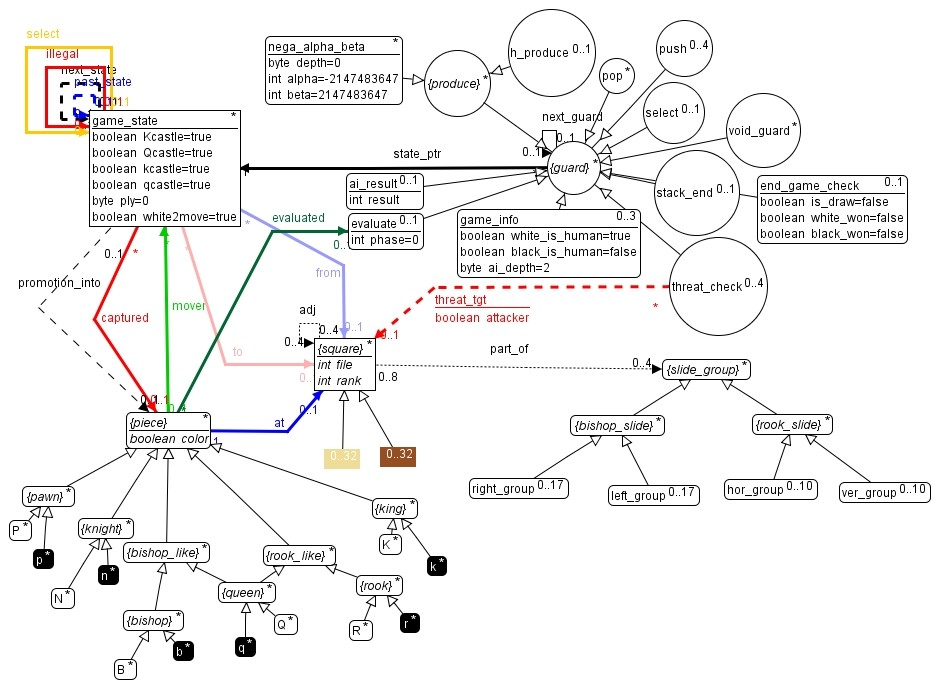
\includegraphics[width=.8\linewidth]{images/type_graph.jpg}
        \caption{The type graph of the system.}
    \end{figure}

    \paragraph{Construction by rules} We could have set up the board by hand (as we actually do to position the pieces and starting the game), but that would have been quite tedious because of the multiple edges needed to make it complete. Instead, we use a set of rules to produce it, which are as follows:
    \begin{itemize}
        \item \texttt{produce\_first\_square} creates a first square of the board (the white top left square, \texttt{file=0} and \texttt{rank=7}), if it has not been created yet. This is then used as a seed for the rest of the construction.
        \begin{figure}[H]
            \centering
            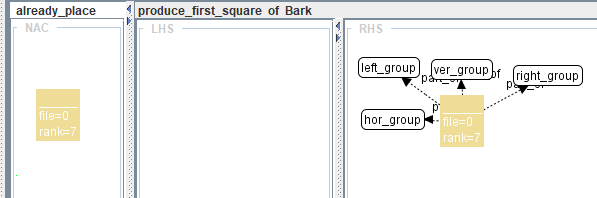
\includegraphics[width=.8\linewidth]{images/produce_first_square.png}
            \caption{\texttt{produce\_first\_square}}
        \end{figure}

        \item \texttt{produce\_top\_rank\_b/w} respectively create black and white squares of the top rank, if the they have not been created yet.
        \begin{figure}[H]
            \centering
            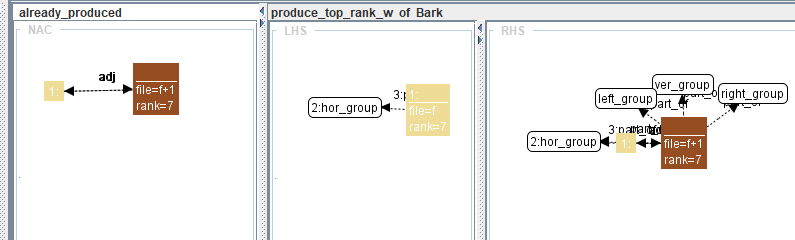
\includegraphics[width=.8\linewidth]{images/produce_top_rank.png}
            \caption{\texttt{produce\_top\_rank}}
        \end{figure}

        \item \texttt{produce\_first\_file\_b/w} respectively create the black and white squares of the first file, if they have not been created yet.
        \begin{figure}[H]
            \centering
            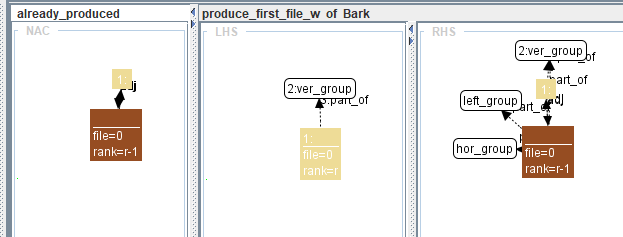
\includegraphics[width=.8\linewidth]{images/produce_first_file.png}
            \caption{\texttt{produce\_first\_file}}
        \end{figure}
    \end{itemize}
    These first rules create the top rank and the left file of the board. The rest of the board is then created by applying:
    \begin{itemize}
        \item \texttt{produce\_square\_b/w} creates a black or white square, if it has not been created yet.
        \begin{figure}[H]
            \centering
            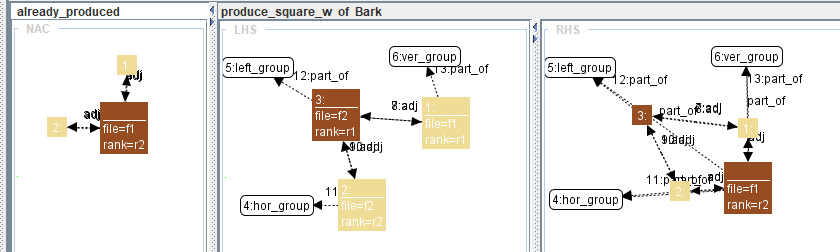
\includegraphics[width=.8\linewidth]{images/produce_square.png}
            \caption{\texttt{produce\_square}}
        \end{figure}

        \item \texttt{add\_right\_group} adds a \noderepr{right\_group} to squares on the last file, if it has not been added yet.
        \begin{figure}[H]
            \centering
            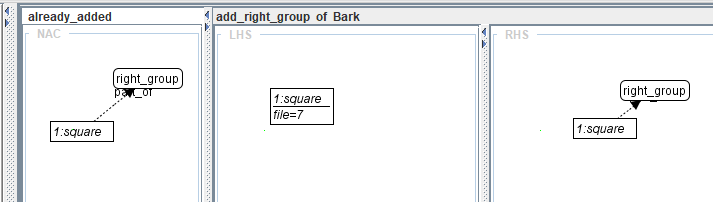
\includegraphics[width=.8\linewidth]{images/add_right_group.png}
            \caption{\texttt{add\_right\_group}}
        \end{figure}

        \item \texttt{produce\_right\_group} connects top-right to bottom-left the squares to the same group, if it has not been done yet.
        \begin{figure}[H]
            \centering
            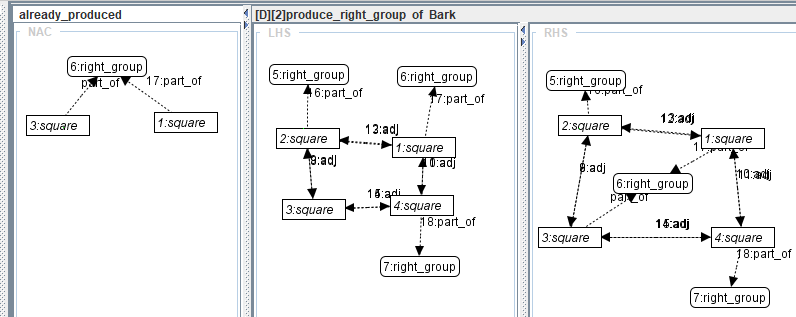
\includegraphics[width=.8\linewidth]{images/produce_right_group.png}
            \caption{\texttt{produce\_right\_group}}
        \end{figure}
    \end{itemize}
    These rules are then applied in a loop until the board is complete.
\end{document}

